\chapter{PHOEBE - Modelo Computacional}

Como se ha planteado, los sistemas binarios estelares ofrecen una oportunidad de
analizar el comportamiento y la estructura estelar que sería imposible deducir
en estrellas aisladas. Sin embargo, el análisis analítico es una herramienta
restringida en cuanto a la cantidad de información que puede extraer de una
curva de luz; las ecuaciones que rigen un sistema binario no tienen una solución
analítica. Para resolver este problema, se hacen códigos capaces de simular la
física de un sistema binario, el cual partiendo de ciertos parámetros estelares
y orbitales pueden reproducir los datos observacionales de un sistema
equivalente en la bóveda celeste.

En el campo de sistemas binarios estelares, uno de los primeros códigos con
mayor impacto es el código \textbf{Wilson-Devinney}, descrito por primera vez en
\autocite{wilson_devinney_realization_of_accurate_binary_lcs_wd_1971}. El código
de Wilson-Devinney\textemdash referenciado como el código \textbf{WD} en varias
publicaciones\textemdash parte del modelo de Roche para representar las
superficies de las estrellas, lo cual le permite hacer un trato adecuado de
fenómenos físicos importantes como el oscurecimiento al limbo y el
oscurecimiento gravitacional. A pesar de sobrepasar 5 décadas de edad el código
WD sigue en uso actualmente en proyectos de investigación (por ejemplo,
\autocite{li_extremely_low_mass_ratio_wd_analysis_2022}), de los cuales se
obtienen los parámetros físicos de un sistema binario estelar observado. Este
trabajo de tesis de maestría utilizó la librería \textbf{PHOEBE}
(\textbf{PH}ysics \textbf{O}f \textbf{E}clipsing \textbf{B}inari\textbf{E}s),
basado en el código WD. En particular se hizo uso de la versión 2.4.11, notando
las varias mejoras realizadas en esta segunda versión mayor en comparación con
versiones menores a 2.0, las cuales utilizaban el código WD como el motor
principal del modelo.

\section{\quotes{Modelo Hacia Adelante}}

El propósito principal de códigos como PHOEBE cae en su capacidad para generar
un \quotes{\textbf{modelo hacia adelante}} (traducido de forma directa de su nombre
en inglés: \textbf{forward model}). Se parte de un modelo del sistema\textemdash
en el caso de un sistema binario, este viene siendo el modelo de Roche junto a
una formulación de las superficies estelares\textemdash el cual se va integrando
en el tiempo, produciendo como resultado datos sintéticos observables como una
curva de luz fotométrica o una curva de velocidades radiales. Un ejemplo de un
sistema \quotes{de juguete} se puede ver en la
\reffigure{figuraPhoebeObservablesSinteticos}. Es importante notar que estos
modelos se trabajan en el espacio fase de la órbita de un sistema; en casos
donde el sistema no experimente algún cambio significativo a lo largo del
tiempo, es suficiente computar el modelo para cada fase orbital observada, dado
que una campaña de observación adecuada abarcaría las mismas fases orbitales más
de una vez.

\begin{figure}[!ht]
	\centering
	\xincludegraphics[scale=0.253, label=\textbf{a)}, labelbox=true, pos=nw, fontsize=\Large]{Introduccion/Figures/Figura PHOEBE LC Sintetico.png}
	\xincludegraphics[scale=0.253, label=\textbf{b)}, labelbox=true, pos=nw, fontsize=\Large]{Introduccion/Figures/Figura PHOEBE RVs Sintetico.png}
	\caption{Datos sintéticos generados usando PHOEBE. Estas curvas representan
	un sistema binario separado, donde $M_1 = 1.0 \ \mathrm{M}_{\odot}$, $M_2 =
	0.5 \ \mathrm{M}_{\odot}$, $R_1 = 2.0 \ \mathrm{R}_{\odot}$, $R_2 = 1.2 \
	\mathrm{R}_{\odot}$, $T_1 = T_2 = 6000 \ \mathrm{K}$, inclinación
	$i_{\mathrm{orb}} = 90^{\circ}$ y periodo orbital $P_{orb} = 1.0 \
	\mathrm{d}$ en una órbita sincrónica. La figura muestra dos diferentes tipos
	de observables: \textbf{a)} Curva de luz fotométrica, cuyas variaciones se
	deben a los eclipses en el sistema. \textbf{b)} Curva de velocidades
	radiales de ambas componentes, donde el movimiento de las estrellas
	individuales a lo largo de nuestra línea de visión causa fluctuaciones
	debido al efecto de Doppler.} 
	\label{figuraPhoebeObservablesSinteticos}
\end{figure}

Para generar datos sintéticos observables de un sistema binario, es necesario
que PHOEBE tome ciertos aspectos en consideración, descritos a continuación en
este capitulo.

\subsection{Discretización de la Superficie Estelar}

Partiendo del modelo de Roche es como se determina la superficie de ambas
componentes, siguiendo el principio de superficies equipotenciales. Sin embargo,
una descripción analítica de las variaciones de las propiedades estelares
resultaría en una complejidad de tiempo intratable del problema; a pesar de
permitirnos modelar pequeñas variaciones en los valores de cada parámetro
superficial, este no es una opción realista dado la capacidad de computo actual.
Es por esto que PHOEBE implementa un método el cual aproxima la superficie de
las estrellas a un muestreo uniforme de puntos determinados por el modelo de
Roche. Sin embargo, se requiere un tratamiento adicional del modelo de Roche; la
\refequation{ecuacionRocheExcentricaAsincronica} viene definida en coordenadas
esféricas, lo cual causaría una distribución no uniforme en el tamaño de los
elementos superficiales no deseada (aparte de causar un tipo de \quotes{costura}
a lo largo del ecuador de la estrella \citetbookchapter{phoebeScientificReference}{5.1.1}).

Para resolver este problema, se transforma la
\refequation{ecuacionRocheExcentricaAsincronica} a un sistema de coordenadas
cilíndrico de acuerdo a las siguientes transformaciones:

\begin{eqfloat}[!ht]
	\centering
	\begin{equation}
		\begin{split}
			& x = \varrho_{\perp} \cos{\phi} \\
			& y = \varrho_{\perp} \sin{\phi} \\
			& z = z
		\end{split}
	\end{equation}
\end{eqfloat}

Donde $\phi$ representa la longitud, $\varrho_{\perp}$ es la componente en el
plano orbital de la distancia al elemento superficial, y $z$ mantiene su
definición del sistema de coordenadas cartesianas. Utilizando estas
transformaciones se llega a una expresión del potencial de Roche en coordenadas
cilíndricas:

% TODO: new page to group equation and text together
\newpage

\begin{eqfloat}[!ht]
	\centering
	\begin{equation}
		\Omega = \frac{1}{\sqrt{\varrho_{\perp} + z^2}} + q \left(\frac{1}{\sqrt{\delta^2 + \varrho_{\perp}^2 + z^2 - 2 \varrho_{\perp} \delta \cos{\phi}}} - \frac{\varrho_{\perp} \cos{\phi}}{\delta^2} \right) + \frac{F^2 \left(1 + q\right) \varrho_{\perp}^2}{2}
	\end{equation}
	\blankcaption
	\label{ecuacionRocheCilindrica}
\end{eqfloat}

Parecido a la \refequation{ecuacionRadioPolarEstelarEquivalencia} se puede
llegar a una expresión similar para encontrar el valor de $\varrho_{\perp}$ que
le corresponde a los valores dados de $\phi$ y $z$, utilizando un método para
encontrar raíces como el de \textit{Newton-Raphson}:

\begin{eqfloat}[!ht]
	\centering
	\begin{equation}
		\begin{split}
			f(\varrho_{\perp}) = \eqnmark[MyDarkRed]{omega}{\frac{1}{\sqrt{\varrho_{\perp} + z^2}} + q \left(\frac{1}{\sqrt{\delta^2 + \varrho_{\perp}^2 + z^2 - 2 \varrho_{\perp} \delta \cos{\phi}}} - \frac{\varrho_{\perp} \cos{\phi}}{\delta^2} \right) + \frac{F^2 \left(1 + q\right) \varrho_{\perp}^2}{2}} \\
			\eqnmark[MyDarkBlue]{omegaPol}{- \frac{1}{z_{\textrm{pol}}} - \frac{q}{\sqrt{z_{\textrm{pol}}^2 + \delta^2}}}
		\end{split}
	\end{equation}
	\annotate[yshift=-0.3em]{below, left}{omega}{Potencial de Roche $\Omega$}
	\annotate[yshift=-0.2em]{below, left}{omegaPol}{Potencial de referencia en el polo $\Omega_{\mathrm{pol}}$}
	\blankcaption
	\vspace{0.4em}
	\label{ecuacionRadioCilindrica}
\end{eqfloat}

Donde se define $z_{\mathrm{pol}} \equiv \varrho_{\mathrm{pol}}$ como el valor
de referencia del radio al polo de la estrella
\citetbookchapter{phoebeScientificReference}{5.1.1}. Al hacer uso de la derivada
$f\prime (\varrho_{\perp})$\textemdash la cual se puede obtener como lo muestra
\citetbookchapter{phoebeScientificReference}{5.1.1}\textemdash es posible
implementar un método para encontrar las raíces de esta ecuación. El muestreo de la superficie se hace a intervalos regulares de latitud y longitud:

\begin{eqfloat}[!ht]
	\centering
	\vspace{0.6em}
	\begin{equation}
		\begin{split}
			& \eqnmark[MyDarkGreen]{lat}{\theta_k} = \frac{\pi \left(k - 0.5\right)}{2 N} \\
			& \eqnmark[MyLightBlue]{lon}{\phi_l} = \frac{\pi \left(l + \left[(l + 1) \textrm{mod} \ 2\right] \div 2 \right)}{M_k}
		\end{split}
	\end{equation}
	\annotate[yshift=1.1em]{above, left}{lat}{Latitud}
	\annotate[yshift=-0.2em]{below, left}{lon}{Longitud}
	\vspace{0.4em}
\end{eqfloat}

Donde $N$ es el número de elementos superficiales solicitados en la muestra. Se
define los subindices $k = 1 \dots N$ y $l = 1 \dots M_k$, donde $M_k := 1 +
\mathrm{int}\left(1.3 N \sin{\theta_k}\right)$
\citetbookchapter{phoebeScientificReference}{5.1}. Una vez que se obtienen las
posiciones de cada muestra se adopta una forma tal que forme una \quotes{malla}
que representa la superficie estelar. Cada elemento de la malla se considera
uniforme con respecto a sus propiedades, como su temperatura efectiva, gravedad
superficial, el radio local, etc. En PHOEBE v2.0 y en adelante se utilizan
elementos en forma de triángulos equiláteros, tal como se muestra en la
\reffigure{figuraMallaPhoebe}. 

\begin{figure}[!ht]
	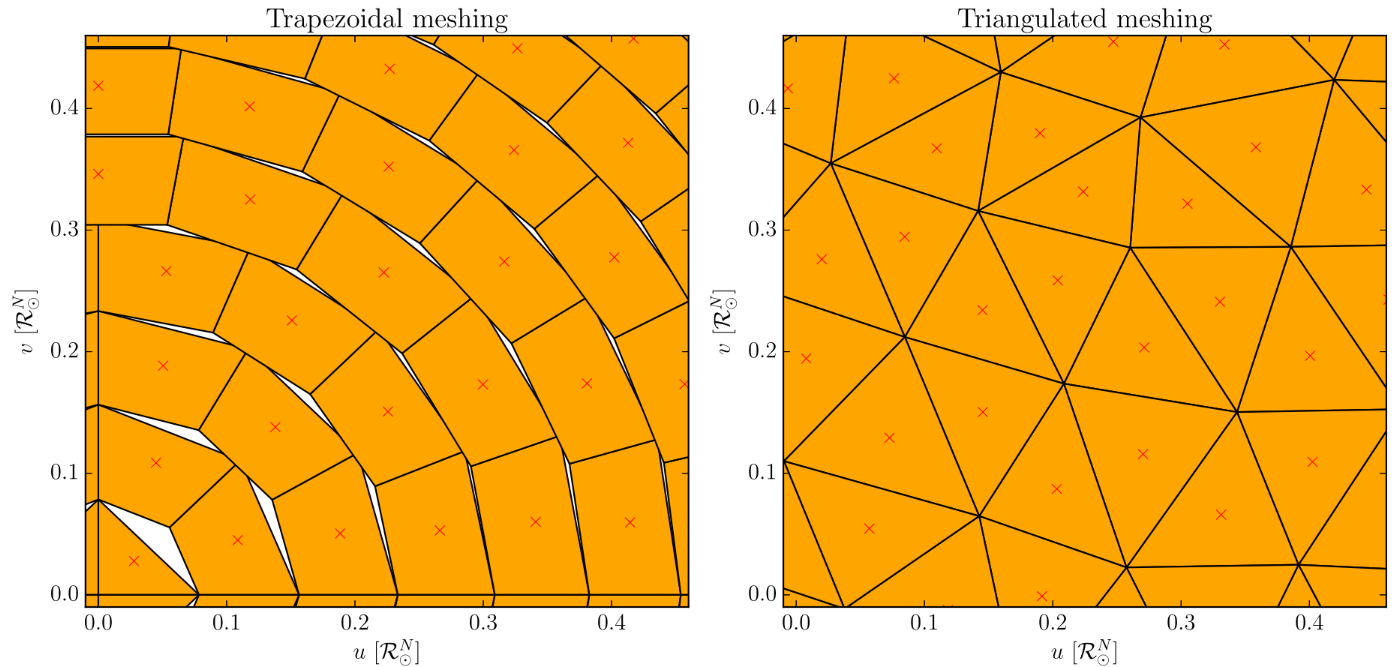
\includegraphics[scale=0.45]{Introduccion/Figures/Figura Mallado Triangular_PHOEBE II Mesh.png}
	\caption{Comparación la discretización superficial usando elementos
	trapezoidales vs. triangulares en el polo estelar. Al utilizar elementos de
	área superficial idéntica se nota que en el caso de elementos trapezoidales
	llega a haber huecos en la superficie que se manifiestan en errores
	sistemáticos en las curvas sintéticas generadas por el modelo, debido a la
	contribución nula de estas fallas en la malla. Estos errores se ven más
	pronunciados entre mayor sea la distorsión experimentada por la estrella. Al
	utilizar elementos en forma de triángulos equiláteros se puede observar que
	se obtiene una superficie continua, eliminando esta fuente de error en el
	modelo. Figura obtenida de
	\autocite{prsa_phoebe_increased_model_fidelity_mesh_2016}}
	\label{figuraMallaPhoebe}
\end{figure}

Esta malla de la superficie estelar se puede ver por completo en la
\reffigure{figuraPhoebeMalla}, donde los parámetros del sistema causan una
distorsión apreciable de ambas estrellas debido a las fuerzas de marea en juego.

\begin{figure}[!ht]
	\centering
	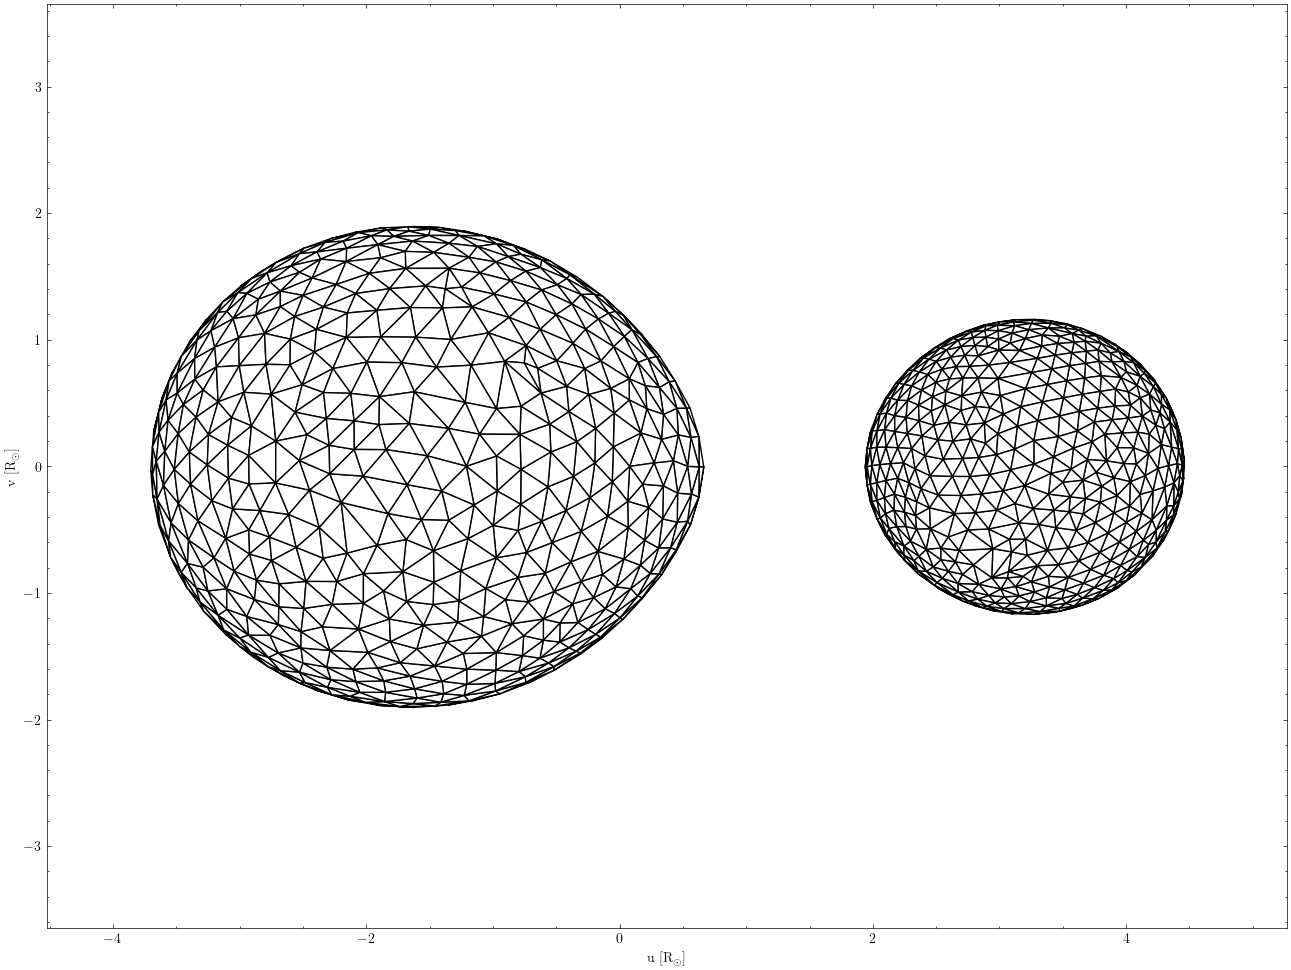
\includegraphics[scale=0.42]{Introduccion/Figures/Figura PHOEBE Malla.png}
	\caption{Mallas de las superficies estelares de un sistema simulado con
	PHOEBE, utilizando los mismos parámetros del modelo utilizado en la
	\reffigure{figuraPhoebeObservablesSinteticos}.}
	\label{figuraPhoebeMalla}
\end{figure}

La malla, al igual que la superficie estelar, no es un objeto constante; en el
caso de un sistema binario de órbita excéntrica las fuerzas de marea que causan
estas distorsiones elipsoidales son dependientes de la fase orbital. A lo largo
de la órbita del sistema, el campo del potencial de Roche va cambiando debido a
la distancia no constante entre ambas componentes estelares. Uno de los
principios del modelo de Roche es que las superficies estelares se ajustan al
campo de fuerzas instantáneo del sistema, el cual va cambiando a escalas de
tiempo significativamente menores que el periodo orbital
\autocite{prsa_phoebe_increased_model_fidelity_mesh_2016}. Esto causaría un
cambio apreciable en los radios estelares, debido a que las superficies
equipotenciales del campo no son constantes en volumen. En teoría, si una
estrella se rige a solo las superficies equipotenciales del mismo valor en cada
fase orbital, la estrella debería de comprimirse o expandirse, irradiando parte
de su energía a su ambiente exterior, llegando rápidamente a una órbita
circular. Sin embargo, esto no es un fenómeno que se ha observado en la
literatura; al contrario, existen sistemas como las estrellas \quotes{heartbeat}
(nombrado por su parecido a una lectura de un electrocardiograma) cuya
variabilidad se debe a la distorsión de sus superficies por fuerzas de marea en
órbitas excéntricas
\autocite{thompson_class_eccentric_binaries_tidal_distortion_heartbeat_2012}.
Como consecuencia, PHOEBE adopta un mecanismo para preservar el volumen del
sistema; al momento de muestrear la superficie para generar la malla
superficial, PHOEBE elige la superficie equipotencial que más se acerque al
volumen calculado de las estrellas en su punto de periastro, el punto en donde
experimentan la mayor distorsión superficial.

\subsection{Distribución de Parámetros Superficiales}

Una estrella no es perfectamente uniforme en la superficie; un modelo acertado
de una estrella debe tomar en cuenta la distribución de parámetros como su
temperatura, intensidad, etc. Para esto se debe calcular la gravedad superficial
en el polo estelar:

\begin{eqfloat}[!ht]
	\centering
	\begin{equation}
		\textbf{g}_{\textrm{pol}} = -\frac{G m_1}{r_{\textrm{pol}}^2} \frac{\textbf{r}_{\mathrm{pol}}}{r_{\mathrm{pol}}} - \frac{G m_2}{h^2} \frac{\textbf{h}}{h} - \omega^2(t) d_{\perp,\textrm{rot}} \frac{\textbf{d}_{\perp,\textrm{rot}}}{d_{\perp,\textrm{rot}}} 
	\end{equation}
\end{eqfloat}

Donde se define $r_{\mathrm{pol}}$ como el radio al polo estelar, $h =
\sqrt{r_{\mathrm{pol}}^2 + d^2}$ es la distancia del polo estelar al centro de
la estrella compañera, $\omega(t)$ es la velocidad angular como función del
tiempo, y $d_{\perp,\textrm{rot}}$ es la distancia del polo estelar hacia el eje
de rotación del sistema (su centro de masa)
\citetbookchapter{phoebeScientificReference}{5.2}. La gravedad superficial
depende de manera indirecta de la fase orbital, debido al ajuste de la estrella
a una superficie equipotencial a lo largo de la órbita del sistema. Este
parámetro rige la distribución de material y energía en la estrella; las
regiones de mayor gravedad superficial (en sistemas binarios eclipsantes suelen
ser los polos estelares, debido a las fuerzas de marea que resultan en un radio
ecuatorial mayor) con áreas más calientes que el resto de la superficie.
\citetbookchapter{phoebeScientificReference}{4.3} dice que el flujo
monocromático para el rango de longitud de onda $[\lambda, \lambda +
\mathrm{d}\lambda]$ es proporcional tanto a la gravedad superficial como a la
temperatura efectiva:

\begin{eqfloat}[!ht]
	\centering
	\begin{equation}
		F_{\lambda} = - \frac{16 \sigma T_{\textrm{eff}}^3}{3 \bar{\kappa} \rho} \frac{\textrm{d}T_{\textrm{eff}}}{\textrm{d}\Omega} g^{\beta}
	\end{equation}
\end{eqfloat}

Donde $\sigma = 5.67 \times 10^{-8} \mathrm{W} \mathrm{m}^{-2} \mathrm{K}^{-4}$
es la constante de Stefan-Boltzmann, $\bar{\kappa}$ es el coeficiente de
opacidad de Rosseland (el cual describe la opacidad, o la probabilidad de un
fotón de atravesar un medio\textemdash en este caso la superficie estelar),
$\rho$ es la densidad del material en la fotosfera, $g$ es la aceleración
gravitacional local, y $\beta$ es el \textit{coeficiente del oscurecimiento
gravitacional}. El valor de $\beta$ en lo general se mantiene fijo dependiendo
de la naturaleza de la envoltura estelar:

\begin{eqfloat}[!ht]
	\centering
	\begin{equation}
		\beta = \left\{\begin{matrix}
			0.32 & \textrm{envoltura convectiva} & T_{\textrm{eff}} < 5000 \ \textrm{K} \\
			1 & \textrm{envoltura radiativa} & T_{\textrm{eff}} > 8000 \ \textrm{K} \\
			\end{matrix}\right. 
	\end{equation}
\end{eqfloat}

Utilizando este coeficiente es posible calcular la temperatura y el flujo de un
elemento superficial dependiendo de la aceleración gravitacional local, dado un
valor de referencia que corresponde al polo estelar:

\begin{eqfloat}[!ht]
	\centering
	\begin{equation}
		\begin{split}
			& F = F_{\textrm{pol}} \left(\frac{g}{g_{\textrm{pol}}}\right)^{\beta} \\
			& T_{\textrm{eff}} = T_{\textrm{eff},\textrm{pol}} \left(\frac{g}{g_{\textrm{pol}}}\right)^{\beta/4}
		\end{split}
	\end{equation}	
\end{eqfloat}

De la cual se obtiene el flujo y la temperatura efectiva dada una aceleración
gravitacional local, donde el término
$\left(g/g_{\mathrm{pol}}\right)^{\beta/4}$ se conoce como la \textbf{corrección
del oscurecimiento gravitacional}. La superficie resuelta con respecto a su
gravedad superficial y temperatura efectiva se puede ver en la
\reffigure{figuraMallaPhoebeTeffLogg}.

\begin{figure}[!ht]
	\centering
	\xincludegraphics[scale=0.27, label=\textbf{(a)}, labelbox=true, pos=nw, fontsize=\Large]{Introduccion/Figures/Figura PHOEBE Malla Logg.png}
	\xincludegraphics[scale=0.27, label=\textbf{(b)}, labelbox=true, pos=nw, fontsize=\Large]{Introduccion/Figures/Figura PHOEBE Malla Teff.png}

	\caption[Distribución de gravedad superficial y temperatura efectiva
	local.]{Malla de una estrella cuyas propiedades son las mismas que el Sol,
	generada utilizando PHOEBE, donde el potencial efectivo es calculado no en
	base al modelo de Roche, si no basado en su frecuencia de rotación, en el
	caso de una estrella singular\textemdash a pesar de que esta información no
	esté documentada explícitamente en un documento fácil de encontrar, esto se
	puede ver en el código fuente de PHOEBE 2, en este caso en el archivo
	\href{https://github.com/phoebe-project/phoebe2/blob/master/phoebe/distortions/rotstar.py}{\code{rotstar.py}}.
	Se puede ver la distribución de gravedad efectiva superficial en el índice
	\textbf{(a)}, al cual se acopla la distribución de temperatura efectiva
	vista en el índice \textbf{(b)}.}
	\label{figuraMallaPhoebeTeffLogg}
\end{figure}

\subsection{Radiación Emergente}

Una vez determinada la distribución de parámetros superficiales es posible
determinar la radiación emergente de cada elemento superficial, del cual se
calcula el flujo que recibe un observador. El flujo de una estrella no es una
cantidad que PHOEBE determina directamente; PHOEBE más bien calcula la
\textit{intensidad}, que se define como la cantidad de energía $\mathrm{d}E$
emitida a través de el ángulo solido $\mathrm{d}\Omega$ por una superficie
proyectada a un ángulo $\mathrm{d}A \cos{\theta}$ en el intervalo de tiempo
$\mathrm{d}t$:

\begin{eqfloat}[!ht]
	\centering
	\begin{equation}
		I_{\lambda} = \frac{\textrm{d}E}{\textrm{d}\lambda \textrm{d}A \cos{\theta} \textrm{d}\Omega \textrm{d}t}
	\end{equation}
	\blankcaption
	\label{ecuacionIntensidadMonocromatica}
\end{eqfloat}

Donde $I_{\lambda}$ es la \textit{intensidad monocromática}, para un intervalo
de longitud de onda $[\lambda, \lambda + \textrm{d}\lambda]$. Esta cantidad es
calculada en la dirección normal de cada elemento superficial; la
\reffigure{figuraMallaPhoebeIntensidadNormal} muestra la distribución de
intensidad absoluta a lo largo de la superficie estelar. La intensidad
monocromática se obtiene partiendo del modelo atmosférico empleado, ya sea el de
cuerpo negro básico o una tabla como la de \autocite{kurucz_atlas_1970}. Para
obtener la \textit{intensidad absoluta} es necesario integrar la intensidad
monocromática sobre todas las longitudes de onda:

\begin{eqfloat}[!ht]
	\centering
	\begin{equation}
		I = \int_{0}^{\infty}{I_{\lambda} \textrm{d}\lambda}
	\end{equation}
	\blankcaption
	\label{ecuacionIntensidadTotal}
\end{eqfloat}

\begin{figure}[!ht]
	\centering
	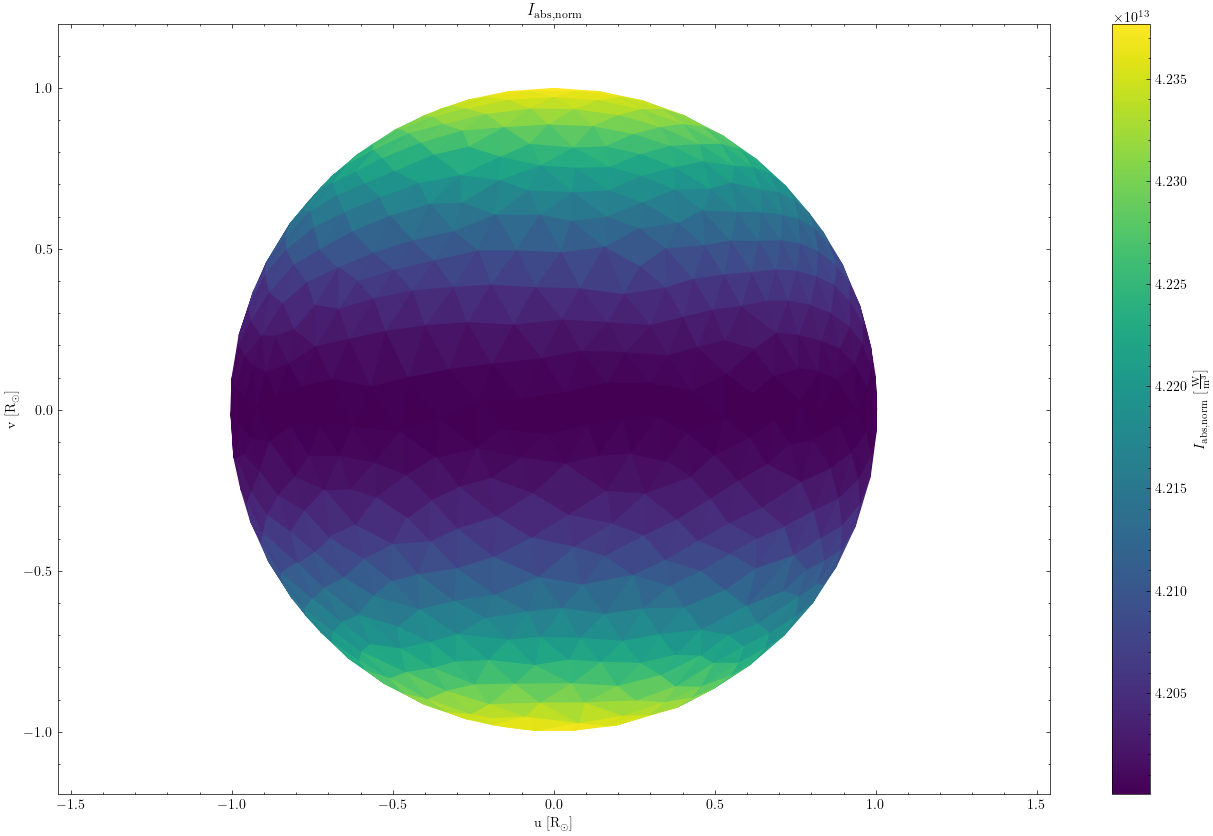
\includegraphics[scale=0.4]{Introduccion/Figures/Figura PHOEBE Malla Intensidad Normal.png}
	\caption{Intensidad absoluta de una estrella modelada utilizando PHOEBE,
	integrada en las longitudes de onda que abarca el pasa banda de
	\textit{Johnson:V}. La figura muestra la intensidad absoluta en la dirección
	del vector normal a los elementos superficiales. Se puede apreciar la
	distribución de la intensidad, la cual sigue el mismo comportamiento de la
	gravedad superficial que se muestra en la
	\reffigure{figuraMallaPhoebeTeffLogg}.}
	\label{figuraMallaPhoebeIntensidadNormal}
\end{figure}

Utilizando la intensidad monocromática definida en la
\refequation{ecuacionIntensidadMonocromatica} se usa para definir la
\textbf{distribución espectral de energía} (\textbf{SED} por sus siglas en
inglés), donde $\mathcal{S} \equiv \mathrm{d}I_{\lambda}/\mathrm{d}\lambda$. El
SED calculado depende tanto en las propiedades de la estrella como en el modelo
empleado para su atmósfera estelar; en el caso de un cuerpo negro, su SED
depende solo de su temperatura efectiva, mientras que modelos como
\autocite{kurucz_atlas_1970} requieren parámetros adicionales como la
metalicidad estelar y gravedad superficial. Sin embargo, en el modelo hacia
adelante de una estrella es de gran importancia determinar la intensidad en una
\textit{pasa banda}; esta es definida por una curva de transmisión, la cual
describe la cantidad de radiación incidente que traspasa el sistema óptico.
PHOEBE tiene varias pasa bandas disponibles, como por ejemplo la de
\textit{Johnson:V} vista en la \reffigure{figuraPhoebePasabandaJohnsonV}.
Utilizando la pasa banda elegida y el SED calculado se computa la intensidad de
la pasa banda con la siguiente ecuación:

\begin{eqfloat}
	\centering
	\begin{equation}
		I_{\textrm{pb}} = \int_{\lambda}{\mathcal{S}(\lambda) \mathcal{P}(\lambda)\textrm{d}\lambda}
	\end{equation}
	\blankcaption
	\label{ecuacionIntensidadPasabanda}
\end{eqfloat}

Donde $I_{\mathrm{pb}}$ como $\mathcal{S}$ son funciones que toman de parámetro
de entrada las propiedades termodinámicas de la estrella, incluyendo incluso
efectos extrínsecos al sistema como la extinción interestelar
\autocite{prsa_phoebe_increased_model_fidelity_mesh_2016}. La intensidad
$I_{\mathrm{pb}}$ definida en la \refequation{ecuacionIntensidadPasabanda} solo
es apropiada para simular un detector calibrado por flujo de estrellas
estándares; para medir la intensidad con respecto al número de fotones
detectados es necesario dividir $I_{\mathrm{pb}}$ entre la energía del fotón
incidente, definida como $E_{\lambda} = hc/\lambda$, e integrar:

\begin{eqfloat}
	\centering
	\begin{equation}
		I_{\textrm{pb}, \textrm{fot}} = \int_{\lambda}{\left(\frac{\mathcal{S}(\lambda) \mathcal{P}(\lambda)}{E_{\lambda}}\textrm{d}\lambda \right)} = \frac{1}{hc} \int_{\lambda}{\lambda \mathcal{S}(\lambda) \mathcal{P}(\lambda) \textrm{d}\lambda}
	\end{equation}
\end{eqfloat}

Por último, se integra $I_{\mathrm{pb}, \mathrm{fot}}$ o $I_{\mathrm{pb}}$\textemdash
dependiendo si se desea el flujo por cuentas de fotones o en energía\textemdash
a lo largo de la superficie estelar visible para obtener el flujo emitido por la
estrella en la pasa banda deseada, llegando como resultado a una curva de luz
sintética como en la \reffigure{figuraPhoebeObservablesSinteticos}, la cual
forma la base del análisis fotométrico de un sistema binario estelar.

\begin{figure}[!ht]
	\centering
	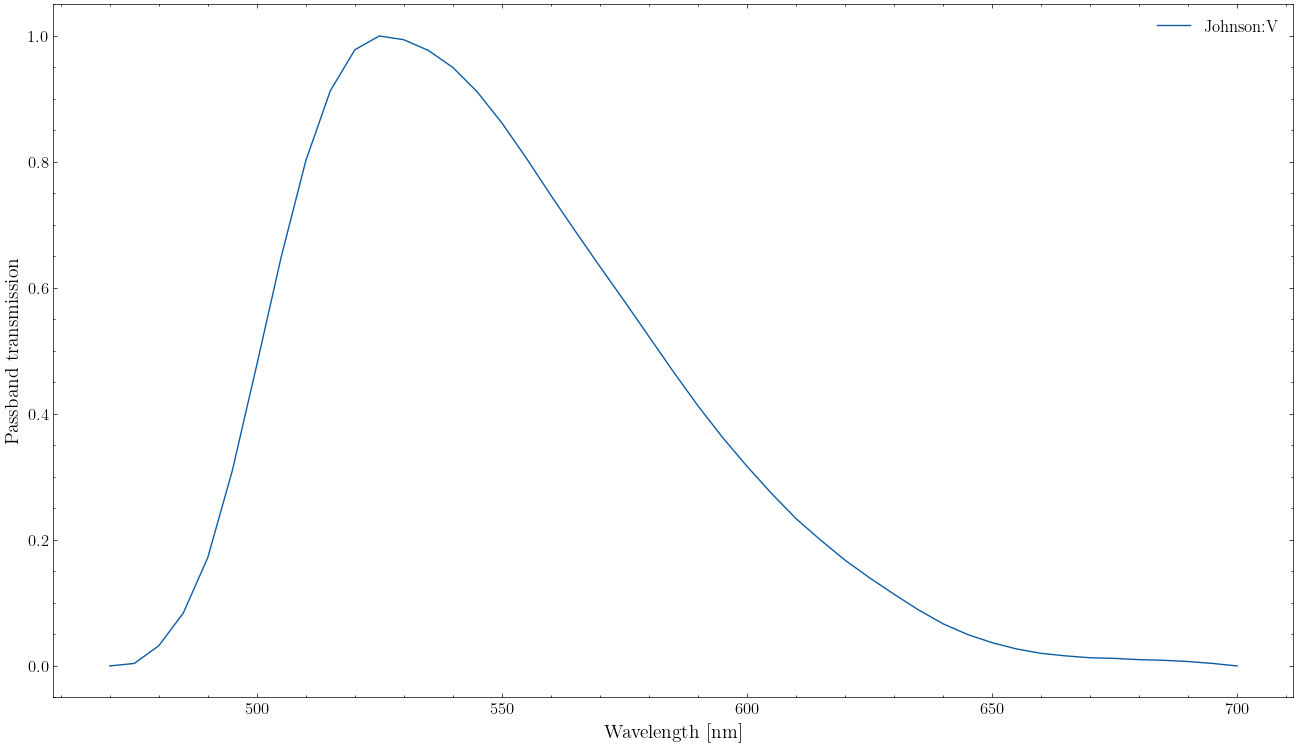
\includegraphics[scale=0.4]{Introduccion/Figures/Figura PHOEBE JohnsonV Pasabanda.png}
	\caption{Curva de transmisión en PHOEBE para la pasa banda \textit{Johnson:V}.}
	\label{figuraPhoebePasabandaJohnsonV}
\end{figure}

\section{El Problema Inverso}

El tener un modelo sofisticado de un sistema binario estelar nos ayuda a
entender los mecanismos responsables por su comportamiento, incluyendo como
afectan las diferentes combinaciones de parámetros estelares en las curvas
observables del sistema. Sin embargo, el propósito de modelos como PHOEBE o WD
yace en determinar los parámetros físicos que, una vez imputadas al modelo,
generan una curva observable sintética que se acopla a datos reales observados
del sistema. Esto en general se conoce como el \textbf{problema inverso}, y es
tanto una gran parte de este trabajo de tesis como el objetivo de varias
investigaciones en la literatura. Encontrar los parámetros que mejor ajustan un
modelo a datos observados es un proceso particular para cada objeto estudiado;
sin embargo, existe un proceso general que se sigue para llegar a una conclusión
cuyos errores y sesgos sean aceptables.

\subsection{Función de Calidad}

Para saber si un modelo es un buen ajusto a una curva observable de un sistema es necesario definir una función que sirva para parametrizar el error entre el modelo sintético y los datos reales. 